\documentclass[aspectratio=169,10pt]{beamer}
\usepackage[utf8]{inputenc}
\usepackage[T1]{fontenc}
\usepackage{lmodern}
\usepackage{graphicx}
\usepackage{booktabs}
\usepackage{amsmath}
\usepackage{xcolor}

\definecolor{navy}{HTML}{16324F}
\definecolor{gold}{HTML}{D7A62A}
\definecolor{teal}{HTML}{2A7F86}
\definecolor{warmgray}{HTML}{F3F1EC}
\definecolor{alertred}{HTML}{A63D40}

\setbeamercolor{normal text}{fg=navy,bg=white}
\setbeamercolor{frametitle}{fg=white,bg=navy}
\setbeamercolor{title}{fg=white}
\setbeamercolor{subtitle}{fg=warmgray}
\setbeamercolor{structure}{fg=teal}
\setbeamercolor{alerted text}{fg=alertred}
\setbeamercolor{block title}{fg=white,bg=teal}
\setbeamercolor{block body}{fg=navy,bg=warmgray}
\setbeamertemplate{navigation symbols}{}
\setbeamertemplate{itemize item}{\color{gold}$\blacktriangleright$}
\setbeamertemplate{itemize subitem}{\color{teal}$\bullet$}
\setbeamertemplate{footline}{%
  \hfill\usebeamerfont{page number in head/foot}\insertframenumber\hspace{0.5cm}\vspace{0.18cm}}
\setbeamersize{text margin left=0.55cm,text margin right=0.55cm}
\setbeamerfont{frametitle}{size=\Large,series=\bfseries}
\setbeamerfont{title}{size=\huge,series=\bfseries}
\setbeamerfont{subtitle}{size=\large}

\graphicspath{{../}}

\newcommand{\casecaption}[1]{\vspace{-0.1cm}{\scriptsize\color{navy}\bfseries #1}\vspace{0.05cm}}
\newcommand{\spectrapair}[3]{%
\begin{frame}{#1}
  \centering
  \includegraphics[width=0.495\linewidth,height=0.58\textheight,keepaspectratio]{results/resonances/A_air_#2deg_TRA.png}\hfill
  \includegraphics[width=0.495\linewidth,height=0.58\textheight,keepaspectratio]{results/resonances/B_SiO2_#2deg_TRA.png}
  \vspace{0.05cm}

  \begin{minipage}{0.97\linewidth}
    \footnotesize #3
  \end{minipage}
\end{frame}}

\newcommand{\fieldslide}[7]{%
\begin{frame}{#1}
  \centering
  \includegraphics[width=0.32\linewidth,height=0.48\textheight,keepaspectratio]{results/nearfields/request_#2_xy.png}\hfill
  \includegraphics[width=0.32\linewidth,height=0.48\textheight,keepaspectratio]{results/nearfields/request_#2_xz.png}\hfill
  \ifnum#2=1\relax
    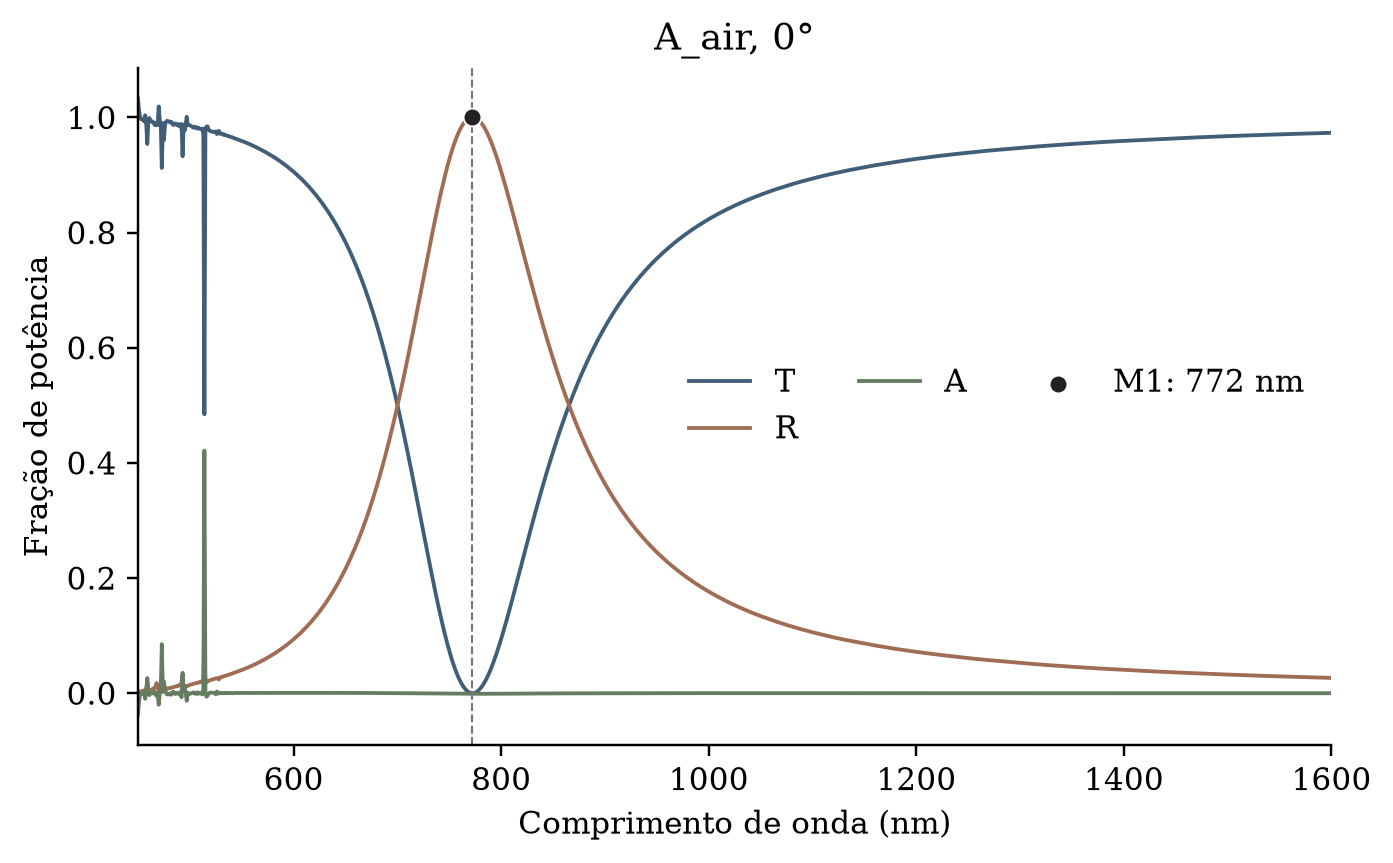
\includegraphics[width=0.32\linewidth,height=0.48\textheight,keepaspectratio]{results/resonances/A_air_0deg_TRA.png}%
  \else\ifnum#2=2\relax
    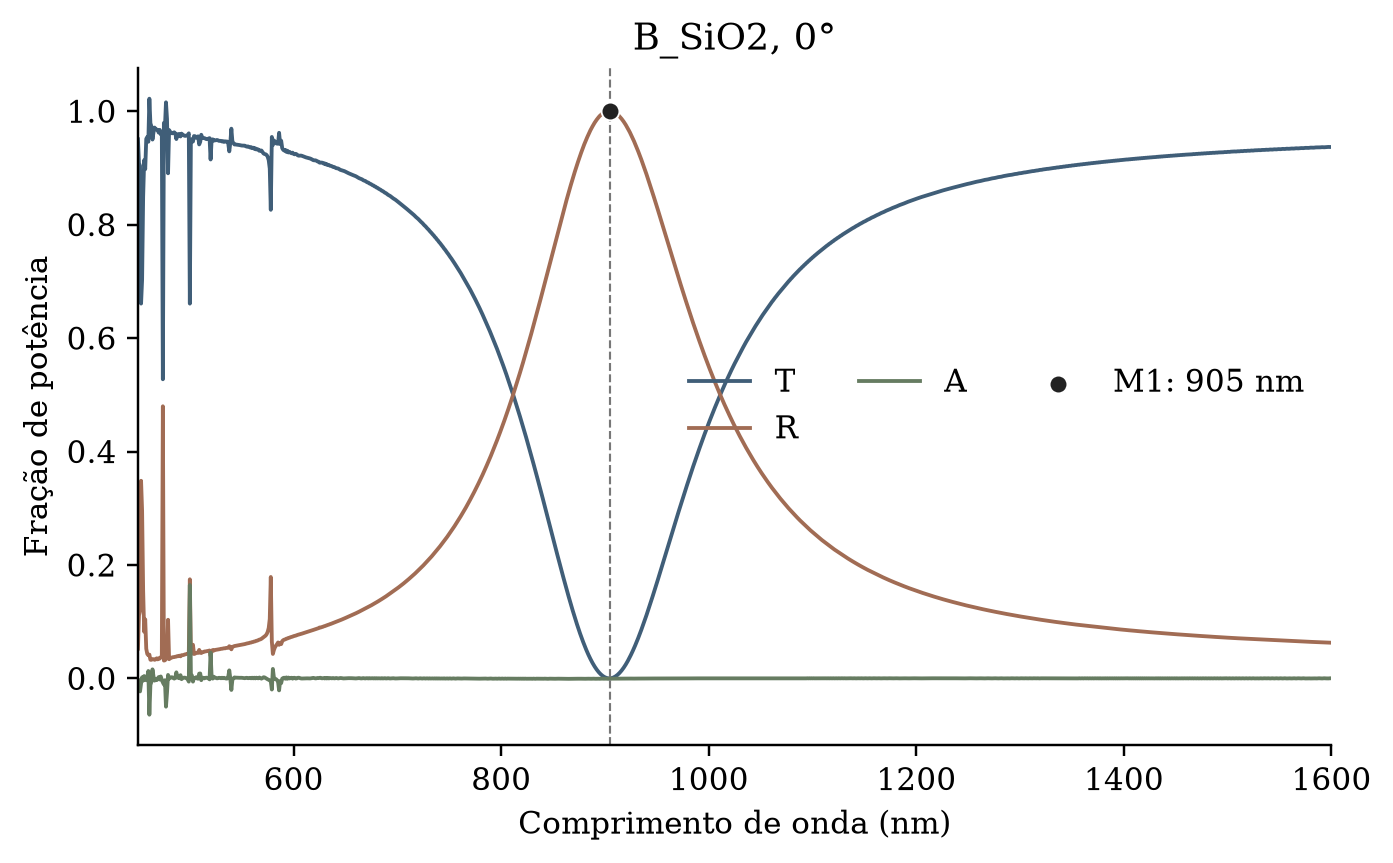
\includegraphics[width=0.32\linewidth,height=0.48\textheight,keepaspectratio]{results/resonances/B_SiO2_0deg_TRA.png}%
  \else\ifnum#2=3\relax
    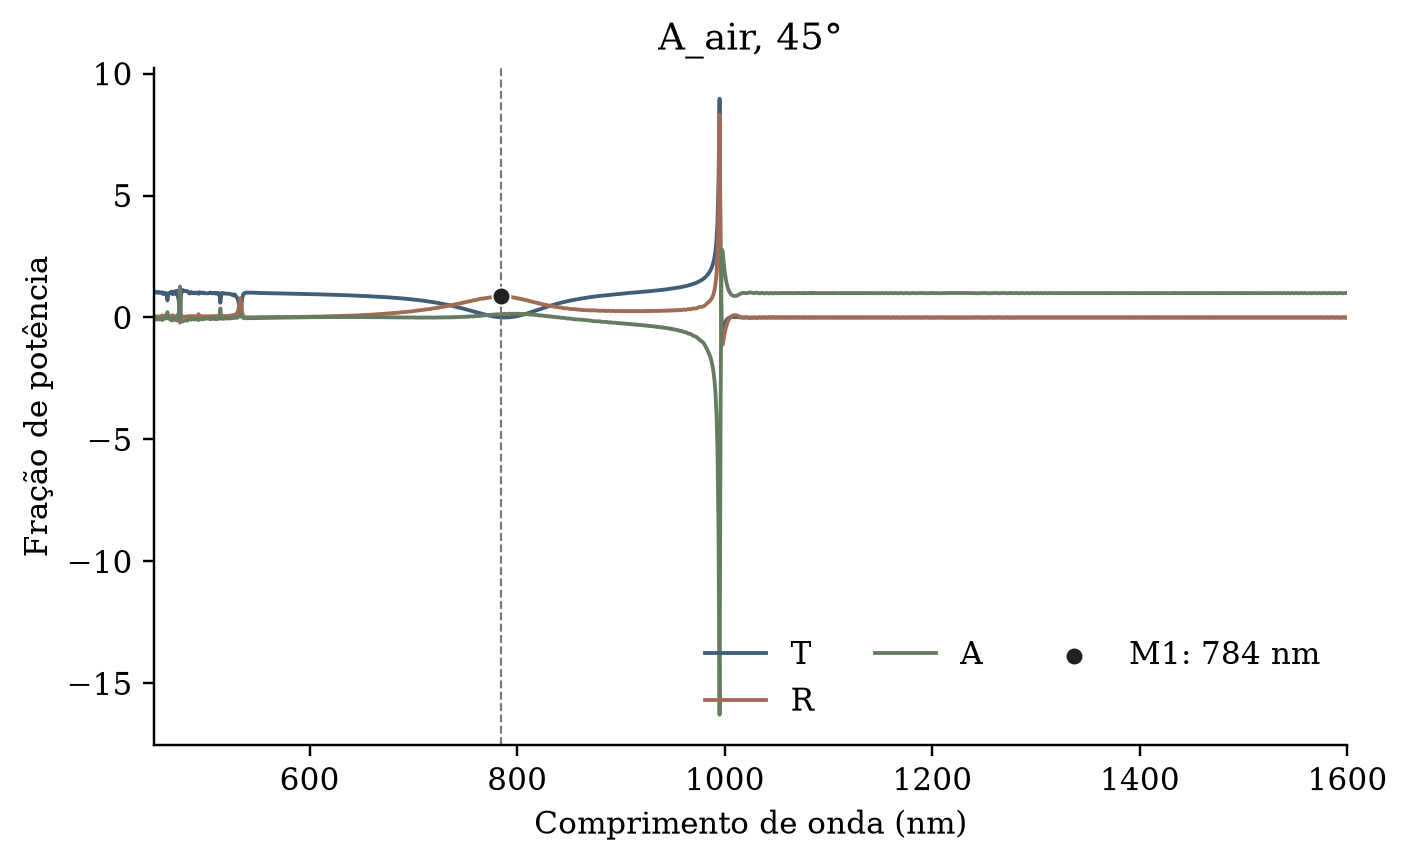
\includegraphics[width=0.32\linewidth,height=0.48\textheight,keepaspectratio]{results/resonances/A_air_45deg_TRA.png}%
  \else
    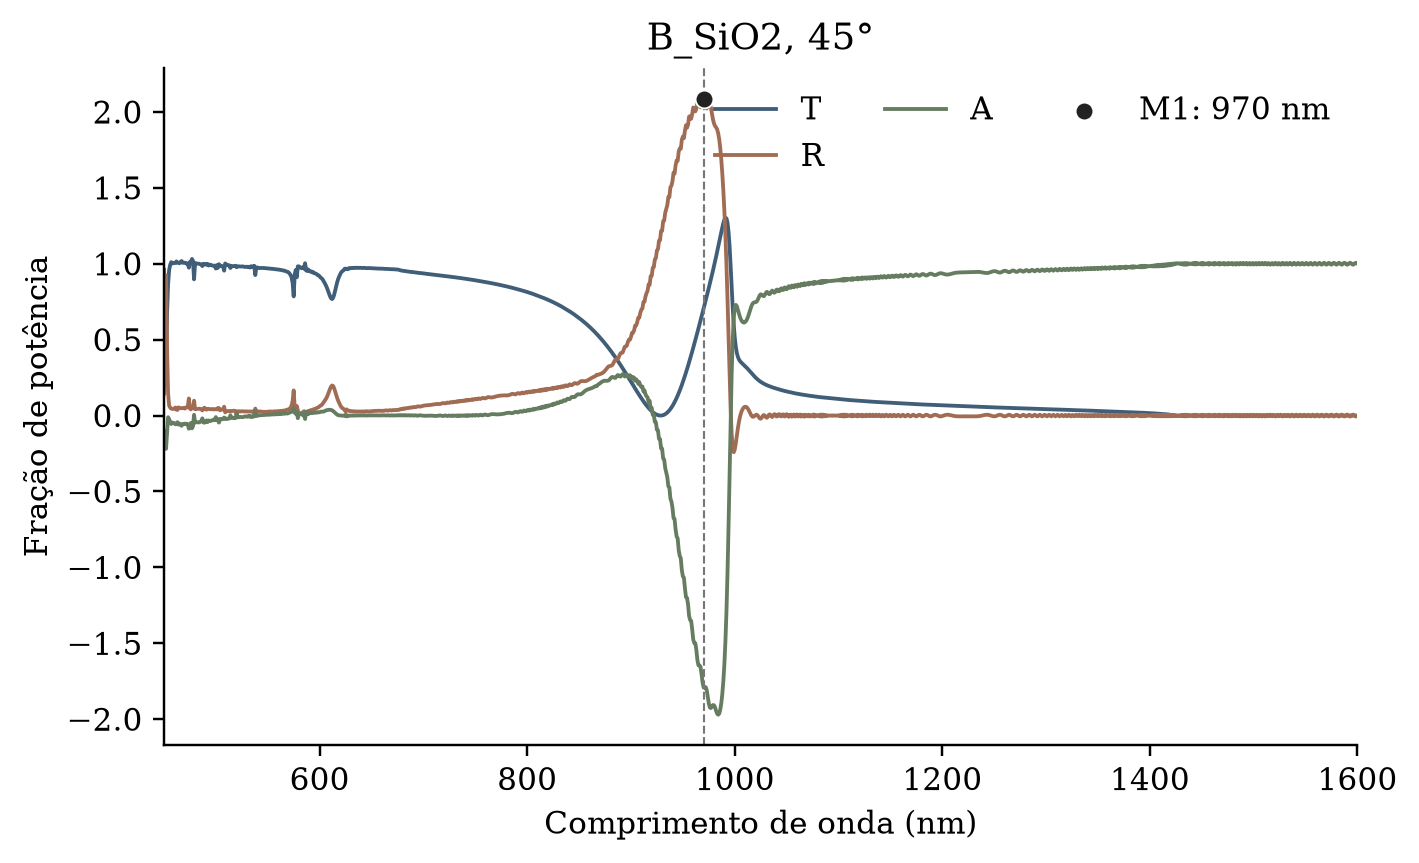
\includegraphics[width=0.32\linewidth,height=0.48\textheight,keepaspectratio]{results/resonances/B_SiO2_45deg_TRA.png}%
  \fi\fi\fi
  \vspace{-0.08cm}

  {\scriptsize\makebox[0.32\linewidth]{Plano XY em $z=35$ nm}\hfill
  \makebox[0.32\linewidth]{Corte XZ em $y=0$}\hfill
  \makebox[0.32\linewidth]{Espectro T/R/A e $\lambda_r$}}
  \vspace{0.08cm}

  \begin{columns}[T,onlytextwidth]
    \begin{column}{0.64\textwidth}
      \footnotesize
      \begin{itemize}\setlength\itemsep{0.15em}
        \item $\lambda_r=#3$ nm, $\theta=#4^\circ$.
        \item #5
        \item #6
      \end{itemize}
    \end{column}
    \begin{column}{0.34\textwidth}
      \begin{block}{Conclusão}
        \footnotesize #7
      \end{block}
    \end{column}
  \end{columns}
\end{frame}}

\begin{document}

\begin{frame}[plain]
  \begin{beamercolorbox}[wd=\paperwidth,ht=\paperheight,dp=0pt]{frametitle}
    \vspace{1.25cm}\hspace{0.8cm}
    \begin{minipage}{0.88\paperwidth}
      {\usebeamerfont{title}\color{white}Metassuperfície plasmônica 2D de nanoanéis de Au\par}
      \vspace{0.35cm}
      {\usebeamerfont{subtitle}\color{warmgray}Espectros T/R/A, ressonâncias e campo próximo\par}
      \vspace{0.75cm}
      {\Large\color{gold}Tarefa 3 \textbar{} casos suspenso em ar e sobre SiO$_2$\par}
      \vfill
      \vspace{0.75cm}
    \end{minipage}
  \end{beamercolorbox}
\end{frame}

\begin{frame}{Problema e geometria simulada}
\begin{columns}[T,onlytextwidth]
  \begin{column}{0.57\textwidth}
    \centering
    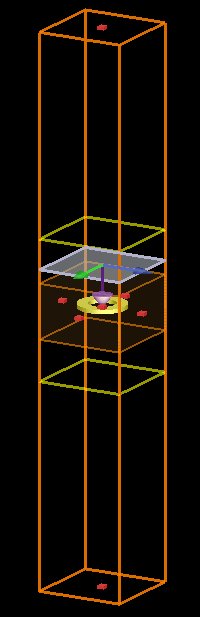
\includegraphics[height=0.67\textheight]{images/air.png}\hspace{0.75cm}
    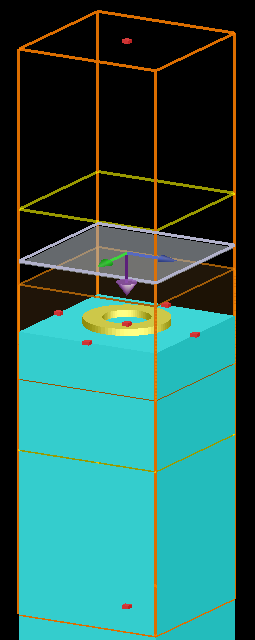
\includegraphics[height=0.67\textheight]{images/glass.png}

    \scriptsize Caso A: ar dos dois lados \hspace{1.0cm} Caso B: substrato de SiO$_2$
  \end{column}
  \begin{column}{0.41\textwidth}
    \small
    \begin{itemize}\setlength\itemsep{0.55em}
      \item Célula unitária quadrada: $P_x=P_y=320$ nm.
      \item Nanoanel de Au: $R_{out}=90$ nm, $R_{in}=50$ nm, largura de 40 nm e altura de 30 nm.
      \item A simulação é 3D; ``2D'' descreve a periodicidade no plano $xy$.
      \item No caso B, o SiO$_2$ atravessa a PML inferior para eliminar uma segunda interface refletora.
      \item Objetivo: comparar como o ambiente dielétrico e o ângulo modificam a resposta óptica.
    \end{itemize}
  \end{column}
\end{columns}
\end{frame}

\begin{frame}{Iluminação e grandezas calculadas}
\begin{columns}[T,onlytextwidth]
  \begin{column}{0.54\textwidth}
    \centering
    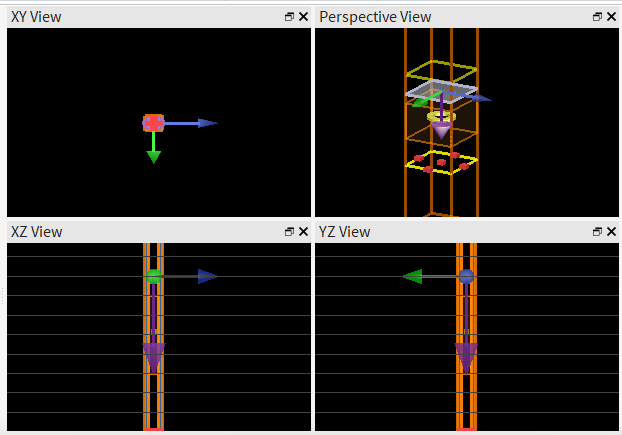
\includegraphics[width=\linewidth,height=0.72\textheight,keepaspectratio]{docs/images/lumerical-perspectiva-elementos.png}
  \end{column}
  \begin{column}{0.44\textwidth}
    \small
    \begin{itemize}\setlength\itemsep{0.48em}
      \item Fonte de onda plana de 450 a 1600 nm, com 1151 pontos: resolução espectral de 1 nm.
      \item Incidência no plano $xz$: $\theta=0,15,30,45,60,75^\circ$, medido a partir da normal $z$.
      \item Polarização TM/p: $\mathbf{E}$ no plano $xz$ e $\mathbf{H}\parallel y$; em $0^\circ$, $\mathbf{E}\parallel x$.
      \item Monitores registram a potência transmitida e refletida, normalizada pela potência incidente.
      \item Em $0^\circ$ usam-se laterais periódicas; nos ângulos oblíquos, Bloch em $x$ e periódica em $y$.
    \end{itemize}
  \end{column}
\end{columns}
\end{frame}

\begin{frame}{Como os monitores calculam T e R}
\begin{columns}[T,onlytextwidth]
  \begin{column}{0.52\textwidth}
    \small
    Os monitores integram o fluxo de potência eletromagnética em seus planos. A potência é normalizada pela potência incidente:
    \vspace{0.2cm}
    \[
      T=\frac{P_{\mathrm{transmitida}}}{P_{\mathrm{incidente}}}
      \qquad
      R=\frac{P_{\mathrm{refletida}}}{P_{\mathrm{incidente}}}
    \]
    \begin{itemize}\setlength\itemsep{0.5em}
      \item Monitor inferior: potência transmitida.
      \item Monitor superior: potência refletida.
      \item Neste projeto, a orientação dos monitores dá $T=-T_{mon}$ e $R=R_{mon}$.
    \end{itemize}
  \end{column}
  \begin{column}{0.45\textwidth}
    \begin{block}{Exemplo ilustrativo}
      \small Se chegam 10 unidades de potência, 6 atravessam e 2 retornam:
      \[
        T=\frac{6}{10}=0{,}6 \qquad R=\frac{2}{10}=0{,}2
      \]
      Assim, 60\% é transmitido e 20\% é refletido. A absorção é $A=1-T-R=0{,}2$.
    \end{block}
    \footnotesize A relação para $A$ requer que toda a potência transmitida e refletida seja contabilizada.
  \end{column}
\end{columns}
\end{frame}

\begin{frame}{Parâmetros numéricos e compromisso de custo}
\begin{columns}[T,onlytextwidth]
  \begin{column}{0.49\textwidth}
    \small
    \begin{itemize}\setlength\itemsep{0.48em}
      \item Ouro dispersivo: \textbf{Au (Gold) - Palik}; SiO$_2$ com $n=1{,}45$.
      \item Domínio FDTD: $z=-800$ a $+800$ nm; PML com 16 camadas e perfil para ângulos rasantes.
      \item Fonte em $z=+300$ nm; reflexão em $+520$ nm; transmissão em $-500$ nm.
      \item Malha local: $3$ nm em $x,y,z$, dentro de $220\times220\times90$ nm ao redor do anel.
    \end{itemize}
  \end{column}
  \begin{column}{0.49\textwidth}
    \small
    \begin{itemize}\setlength\itemsep{0.48em}
      \item Fora da caixa fina: malha automática não uniforme, \emph{mesh accuracy} 2.
      \item Tempo físico máximo: 10 ps; auto-shutoff desejado: $10^{-6}$.
      \item Meta de custo: 30 min por caso $\Rightarrow$ 12 espectros $\approx 6$ h.
      \item Tempo real acumulado nos logs: \alert{$\approx 9{,}64$ h}; alguns casos passaram de 60 min.
      \item Malha mais fina, domínio maior e maior tempo físico tornariam a campanha ainda mais cara.
    \end{itemize}
  \end{column}
\end{columns}
\end{frame}

\begin{frame}{Instabilidade numérica observada}
\begin{columns}[T,onlytextwidth]
  \begin{column}{0.49\textwidth}
    \begin{block}{O que aconteceu}
    \normalsize
    \begin{itemize}\setlength\itemsep{0.55em}
      \item Os 12 espectros chegaram ao limite de 10 ps sem atingir o auto-shutoff de $10^{-6}$.
      \item Restou energia no domínio quando os monitores foram avaliados.
      \item De $30^\circ$ a $75^\circ$, aparecem valores não físicos: $T$, $R$ ou $A$ negativos ou maiores que 1.
    \end{itemize}
    \end{block}
  \end{column}
  \begin{column}{0.49\textwidth}
    \begin{block}{Possível correção e limitação}
    \normalsize
    \begin{itemize}\setlength\itemsep{0.55em}
      \item Seria necessário repetir testes com mais tempo de decaimento, BFAST, malha mais fina e variações de PML/domínio.
      \item A campanha atual já consumiu cerca de 9,64 h; cada refinamento aumentaria muito o custo.
      \item Por isso, não foi possível identificar uma causa única nem demonstrar convergência dentro do prazo disponível.
    \end{itemize}
    \end{block}
  \end{column}
\end{columns}
\vspace{0.15cm}
\centering
\alert{Os resultados oblíquos são apresentados como exploratórios; absorção negativa não tem interpretação física.}
\end{frame}

\begin{frame}{Como interpretar os espectros}
\begin{columns}[T,onlytextwidth]
  \begin{column}{0.56\textwidth}
    \centering
    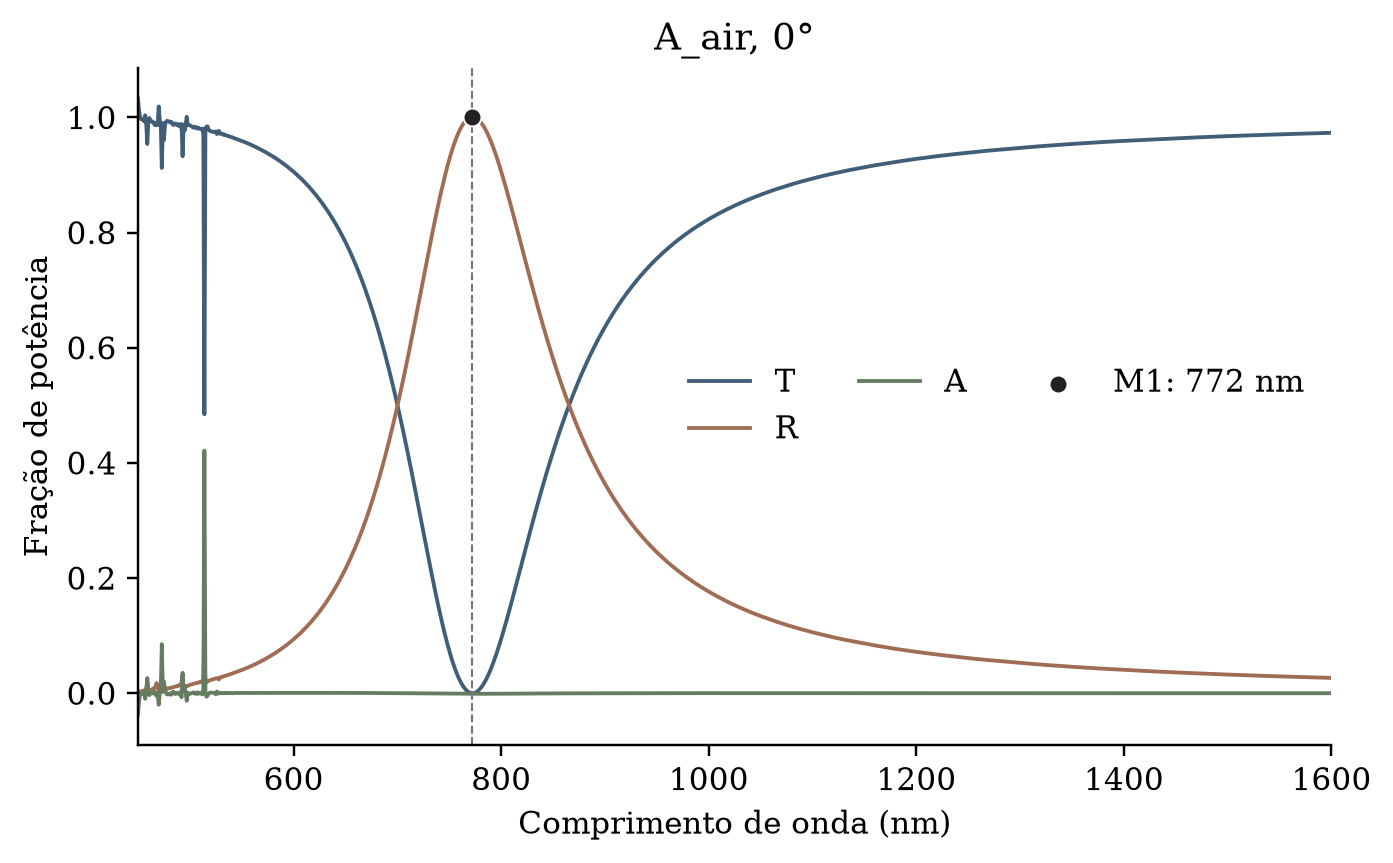
\includegraphics[width=\linewidth,height=0.70\textheight,keepaspectratio]{results/resonances/A_air_0deg_TRA.png}
  \end{column}
  \begin{column}{0.42\textwidth}
    \small
    \begin{itemize}\setlength\itemsep{0.55em}
      \item A ressonância M1 é marcada pela linha tracejada no máximo de $R$ e mínimo de $T$.
      \item Em uma solução física passiva, espera-se $0\le T,R,A\le1$ e $T+R+A=1$.
      \item Valores negativos ou maiores que 1 não representam ganho nem absorção real: são sinais de erro numérico.
      \item Assim, a posição de uma feição suave pode ser discutida; picos estreitos e violações fortes exigem cautela.
    \end{itemize}
  \end{column}
\end{columns}
\end{frame}

\spectrapair{Resultados em incidência normal}{0}{%
  \begin{itemize}\setlength\itemsep{0.35em}
    \item Ar: M1 em \textbf{772 nm}; mínimo profundo de $T$ e máximo de $R$.
    \item SiO$_2$: M1 em \textbf{905 nm}; deslocamento de $+133$ nm.
    \item São os espectros mais coerentes; o maior índice efetivo desloca a resposta para o vermelho.
  \end{itemize}}

\spectrapair{Resultados em 15 graus}{15}{%
  \begin{itemize}\setlength\itemsep{0.35em}
    \item M1 em \textbf{773 nm} no ar e \textbf{908 nm} com SiO$_2$.
    \item Os deslocamentos são de apenas 1 e 3 nm em relação a $0^\circ$.
    \item A feição larga permanece reconhecível, mas as ondulações tornam a análise exploratória.
  \end{itemize}}

\spectrapair{Incidência a 30 graus}{30}{%
  \begin{itemize}\setlength\itemsep{0.35em}
    \item Marcadores: \textbf{776 nm} no ar e \textbf{913 nm} com SiO$_2$.
    \item A estrutura larga de M1 continua próxima da tendência observada até $15^\circ$.
    \item O pico em 1400 nm é artefato: no ar, $A$ chega a aproximadamente $-16{,}6$.
  \end{itemize}}

\spectrapair{Resultados em 45 graus}{45}{%
  \begin{itemize}\setlength\itemsep{0.35em}
    \item Marcadores: \textbf{784 nm} no ar e \textbf{970 nm} com SiO$_2$.
    \item No ar, a feição larga em 784 nm é distinguível, mas há divergência em 1000 nm.
    \item Com SiO$_2$, a feição se mistura a violações de energia; os mapas não corrigem o espectro.
  \end{itemize}}

\spectrapair{Resultados em 60 graus}{60}{%
  \begin{itemize}\setlength\itemsep{0.35em}
    \item Marcadores: \textbf{802 nm} no ar e \textbf{771 nm} com SiO$_2$.
    \item No ar, valores de $R>1$ e $A\ll0$ tornam o ponto pouco confiável.
    \item A mudança abrupta com SiO$_2$ não pode ser atribuída a um modo físico sem convergência.
  \end{itemize}}

\spectrapair{Resultados em 75 graus}{75}{%
  \begin{itemize}\setlength\itemsep{0.35em}
    \item Marcadores: \textbf{726 nm} no ar e \textbf{612 nm} com SiO$_2$.
    \item As curvas exibem grandes regiões com $T>1$ e $A<0$.
    \item A queda contradiz a tendência anterior; os pontos são candidatos, não medidas robustas de M1.
  \end{itemize}}

\begin{frame}{Evolução angular da ressonância selecionada}
\begin{columns}[T,onlytextwidth]
  \begin{column}{0.64\textwidth}
    \centering
    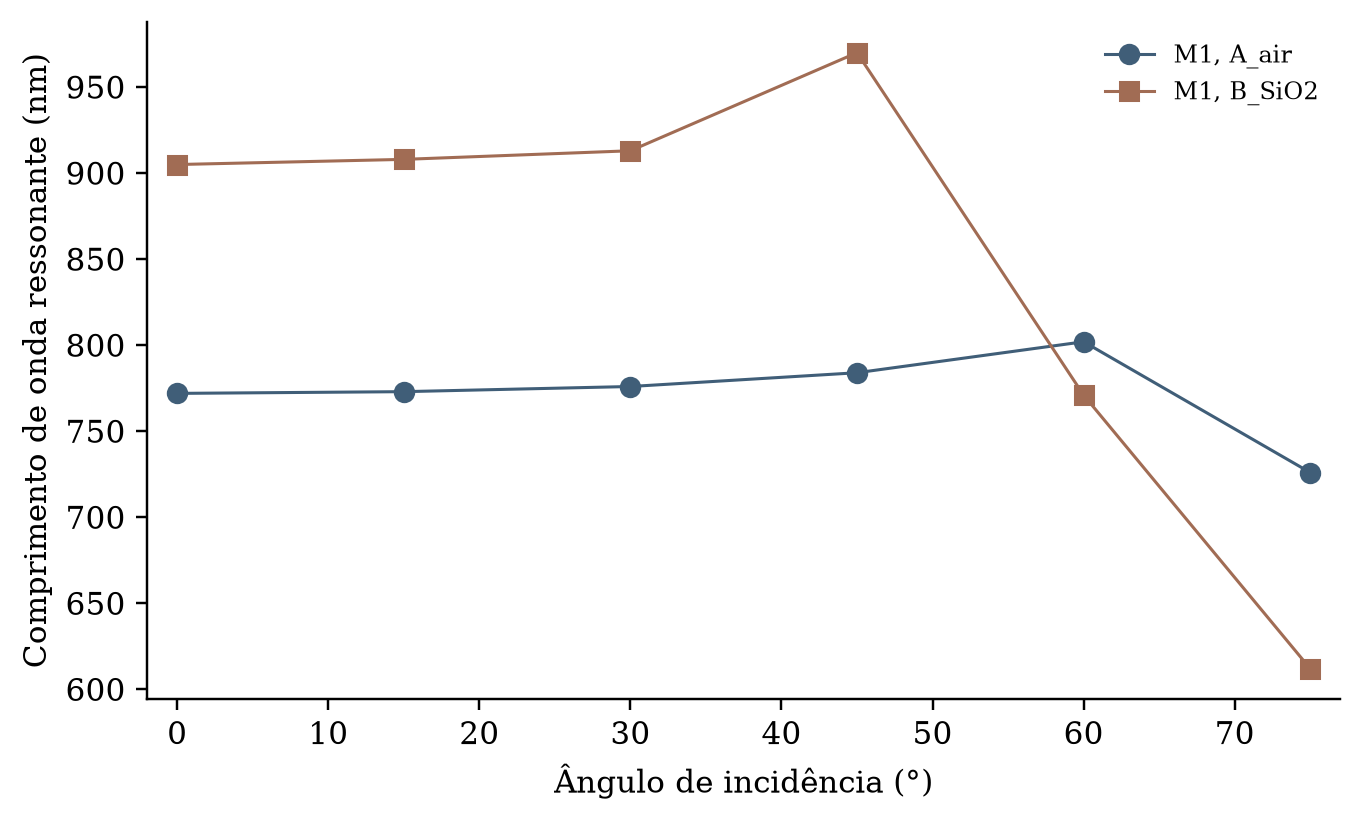
\includegraphics[width=\linewidth,height=0.70\textheight,keepaspectratio]{results/resonances/resonance_vs_angle.png}
  \end{column}
  \begin{column}{0.34\textwidth}
    \scriptsize
    \begin{tabular}{rcc}
      \toprule
      $\theta$ & ar (nm) & SiO$_2$ (nm)\\
      \midrule
      $0^\circ$  & 772 & 905\\
      $15^\circ$ & 773 & 908\\
      $30^\circ$ & 776 & 913\\
      $45^\circ$ & 784 & 970\\
      $60^\circ$ & 802 & 771\\
      $75^\circ$ & 726 & 612\\
      \bottomrule
    \end{tabular}
    \vspace{0.35cm}
    \begin{itemize}\setlength\itemsep{0.42em}
      \item Até $30^\circ$, há evolução suave e deslocamento para o vermelho com o substrato.
      \item A partir de $45^\circ$, a incerteza cresce.
      \item A inversão em $60$--$75^\circ$ coincide com os espectros mais não físicos.
    \end{itemize}
  \end{column}
\end{columns}
\end{frame}

\fieldslide{Campo próximo: ar, $0^\circ$}{1}{772}{0}
{O plano XY mostra hotspots simétricos nas bordas do anel alinhadas com $x$, direção do campo incidente.}
{O corte XZ concentra o campo nos cantos superior e inferior do metal, com máximo visual próximo de $120\,|E_0|^2$.}
{A localização forte e simétrica nas interfaces do Au é compatível com um modo plasmônico dipolar bem excitado.}

\fieldslide{SiO$_2$: campo próximo em $0^\circ$}{2}{905}{0}
{O padrão XY mantém a simetria dipolar, mas a intensidade é menor na escala compartilhada com o caso em ar.}
{No corte XZ, a distribuição é afetada pela interface em $z=0$; os hotspots permanecem nos cantos do anel.}
{O substrato desloca M1 para o vermelho e redistribui o campo, sem alterar a orientação principal do modo.}

\fieldslide{Campo próximo: ar, $45^\circ$}{3}{784}{45}
{O padrão XY ainda é quase simétrico e muito semelhante ao de $0^\circ$, com hotspots nas faces laterais.}
{O corte XZ preserva a localização nos cantos do metal; a componente longitudinal da polarização pode introduzir assimetria discreta.}
{O mapa sustenta a associação do marcador de 784 nm ao mesmo caráter dipolar, mas não valida as regiões divergentes do espectro.}

\fieldslide{SiO$_2$: campo próximo em $45^\circ$}{4}{970}{45}
{O plano XY torna-se assimétrico: o lado de $x<0$ concentra mais intensidade que o lado oposto.}
{O corte XZ também mostra maior localização em uma extremidade, coerente com incidência oblíqua e ambiente assimétrico.}
{Há localização de campo na estrutura, porém a forte instabilidade do espectro impede tratar 970 nm como valor convergido.}

\begin{frame}{Conclusões}
\begin{columns}[T,onlytextwidth]
  \begin{column}{0.58\textwidth}
    \small
    \begin{itemize}\setlength\itemsep{0.6em}
      \item Em incidência normal, M1 é claramente observada em 772 nm no ar e 905 nm sobre SiO$_2$: deslocamento de 133 nm para o vermelho.
      \item Até $30^\circ$, os marcadores evoluem suavemente; nos ângulos maiores, a resposta torna-se numericamente instável.
      \item Os mapas mostram hotspots nas bordas e cantos do anel, evidenciando localização plasmônica de caráter predominantemente dipolar.
      \item O substrato altera simultaneamente a posição espectral, a intensidade e a simetria espacial do campo próximo.
      \item Os resultados de $30$--$75^\circ$ devem ser apresentados como exploratórios, não como solução convergida.
    \end{itemize}
  \end{column}
  \begin{column}{0.40\textwidth}
    \begin{block}{Mensagem final}
      \small A física é mais convincente nos casos em que três evidências concordam: feição suave no espectro, conservação aproximada de energia e campo localizado no nanoanel.
    \end{block}
    \vspace{0.25cm}
    \begin{block}{Próximo passo}
      \small Repetir casos selecionados com BFAST, maior tempo de decaimento e testes de malha/PML antes de quantificar dispersão angular.
    \end{block}
  \end{column}
\end{columns}
\end{frame}

\begin{frame}{HFSS: configuração e parâmetros numéricos}
\begin{columns}[T,onlytextwidth]
  \begin{column}{0.49\textwidth}
    \small
    \begin{itemize}\setlength\itemsep{0.5em}
      \item Mesma geometria, casos em ar e SiO$_2$, ângulos e polarização TM/p.
      \item HFSS Driven Modal, com condições periódicas e portas de Floquet em $z=\pm800$ nm.
      \item Excitação TM$_{00}$ na porta superior. SiO$_2$ com $n=1{,}45$.
      \item Ouro dispersivo: dados Palik importados no HFSS.
    \end{itemize}
  \end{column}
  \begin{column}{0.49\textwidth}
    \small
    \begin{itemize}\setlength\itemsep{0.5em}
      \item Comprimento máximo local no Au: 3 nm. Dez modos por porta no ar e 14 com SiO$_2$.
      \item Adaptação em 374,74 THz: até 20 passes, $\Delta S$ máximo de 0,005 e dois passes convergidos exigidos.
      \item Varredura interpolada: 187,37--666,21 THz, 401 amostras nativas. Resultados reamostrados a cada 1 nm.
      \item $T$ e $R$ somam a potência dos modos propagantes. $A=1-T-R$.
    \end{itemize}
  \end{column}
\end{columns}
\end{frame}

\newcommand{\hfssspectra}[2]{%
\begin{frame}{HFSS: espectros em #1 graus}
  \centering
  \includegraphics[width=0.49\linewidth,height=0.65\textheight,keepaspectratio]{results/hfss_deliverables/resonances/A_air_#1deg_TRA.png}\hfill
  \includegraphics[width=0.49\linewidth,height=0.65\textheight,keepaspectratio]{results/hfss_deliverables/resonances/B_SiO2_#1deg_TRA.png}

  \vspace{0.12cm}
  \begin{minipage}{0.96\linewidth}\footnotesize #2\end{minipage}
\end{frame}}

\hfssspectra{0}{Picos de absorção: ar 1231 nm; SiO$_2$ 483 nm.}
\hfssspectra{15}{Candidatos: ar 1230 nm; SiO$_2$ 494 nm.}
\hfssspectra{30}{Candidatos: ar 451 e 493 nm; SiO$_2$ 550 e 582 nm.}
\hfssspectra{45}{Picos: ar 525, 534 e 550 nm; SiO$_2$ 523, 561, 566, 582, 618, 637 e 659 nm.}
\hfssspectra{60}{Candidatos: ar 547, 579, 595 e 995 nm; SiO$_2$ 569, 575, 582, 586 e 705 nm.}
\hfssspectra{75}{Candidatos: ar 545, 550, 603, 618 e 1003 nm; SiO$_2$ 535, 551, 566, 582, 618, 705 e 758 nm.}

\newcommand{\hfssfield}[5]{%
\begin{frame}{HFSS: campo próximo, #1, $#2^\circ$}
  \centering
  \includegraphics[width=0.32\linewidth,height=0.48\textheight,keepaspectratio]{results/hfss_deliverables/nearfields/#3_#2deg_#4_#5_xy.png}\hfill
  \includegraphics[width=0.32\linewidth,height=0.48\textheight,keepaspectratio]{results/hfss_deliverables/nearfields/#3_#2deg_#4_#5_xz.png}\hfill
  \includegraphics[width=0.32\linewidth,height=0.48\textheight,keepaspectratio]{results/hfss_deliverables/resonances/#3_#2deg_TRA.png}

  {\scriptsize\makebox[0.32\linewidth]{Plano XY em $z=35$ nm}\hfill
  \makebox[0.32\linewidth]{Corte XZ em $y=0$}\hfill
  \makebox[0.32\linewidth]{Espectro do caso}}
  \vspace{0.2cm}
  \begin{columns}[T,onlytextwidth]
    \begin{column}{0.62\textwidth}
      \small
      \begin{itemize}
        \item Candidato #4: $\lambda=#5$ nm, $\theta=#2^\circ$.
        \item Mapas mostram $|E|^2/|E_0|^2$, com referência sem anel.
      \end{itemize}
    \end{column}
  \end{columns}
\end{frame}}

\hfssfield{ar}{0}{A_air}{A01}{1231}
\hfssfield{SiO$_2$}{0}{B_SiO2}{A01}{483}
\hfssfield{ar}{45}{A_air}{A01}{525}
\hfssfield{ar}{45}{A_air}{A02}{534}
\hfssfield{ar}{45}{A_air}{A03}{550}
\hfssfield{SiO$_2$}{45}{B_SiO2}{A01}{523}
\hfssfield{SiO$_2$}{45}{B_SiO2}{A02}{561}
\hfssfield{SiO$_2$}{45}{B_SiO2}{A03}{566}
\hfssfield{SiO$_2$}{45}{B_SiO2}{A04}{582}
\hfssfield{SiO$_2$}{45}{B_SiO2}{A05}{618}
\hfssfield{SiO$_2$}{45}{B_SiO2}{A06}{637}
\hfssfield{SiO$_2$}{45}{B_SiO2}{A07}{659}

\begin{frame}{Comparação: espectros em incidência normal}
\begin{columns}[T,onlytextwidth]
  \begin{column}{0.49\textwidth}\centering
    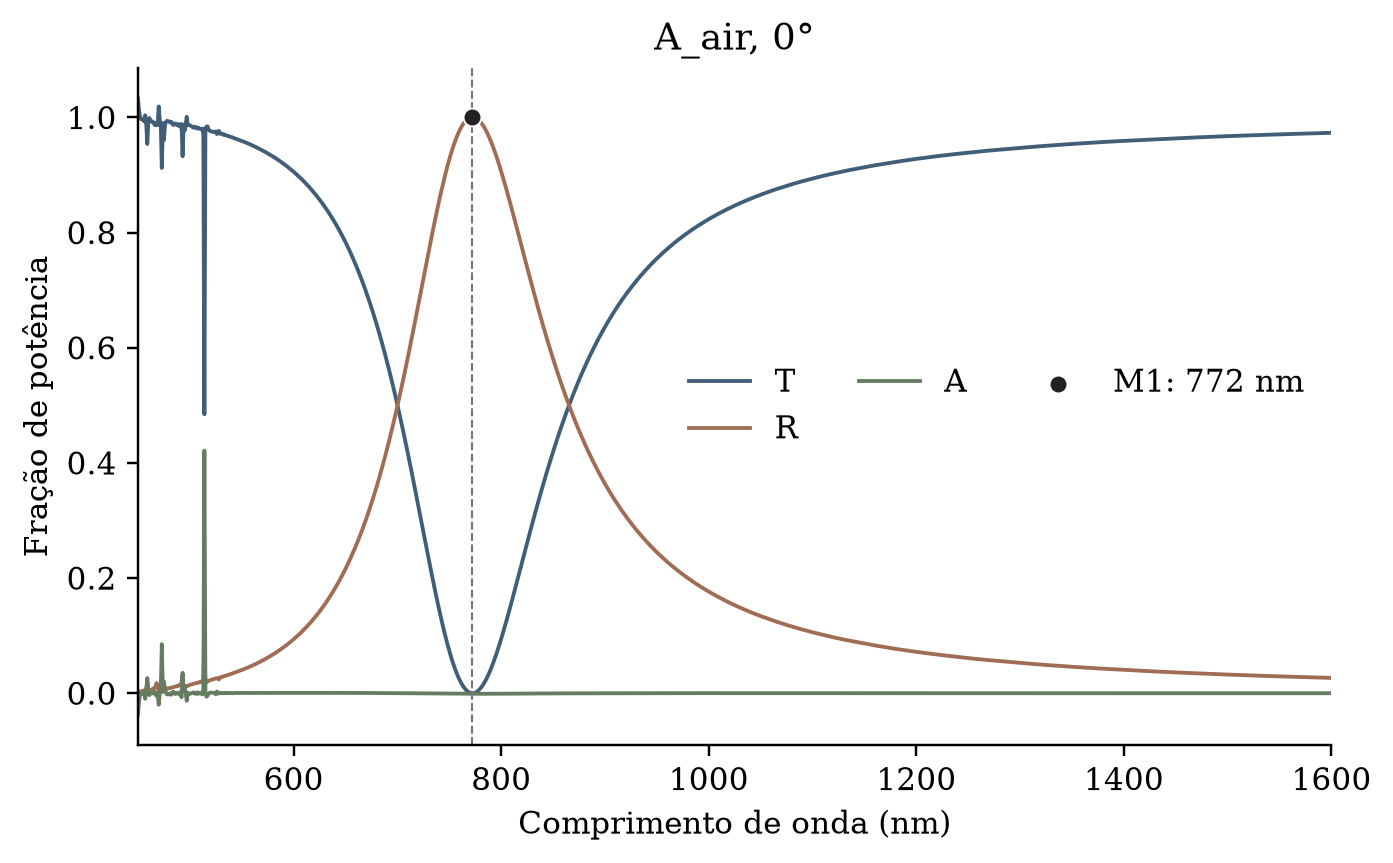
\includegraphics[width=\linewidth,height=0.50\textheight,keepaspectratio]{results/resonances/A_air_0deg_TRA.png}
    \small Lumerical FDTD: ar, $0^\circ$
  \end{column}
  \begin{column}{0.49\textwidth}\centering
    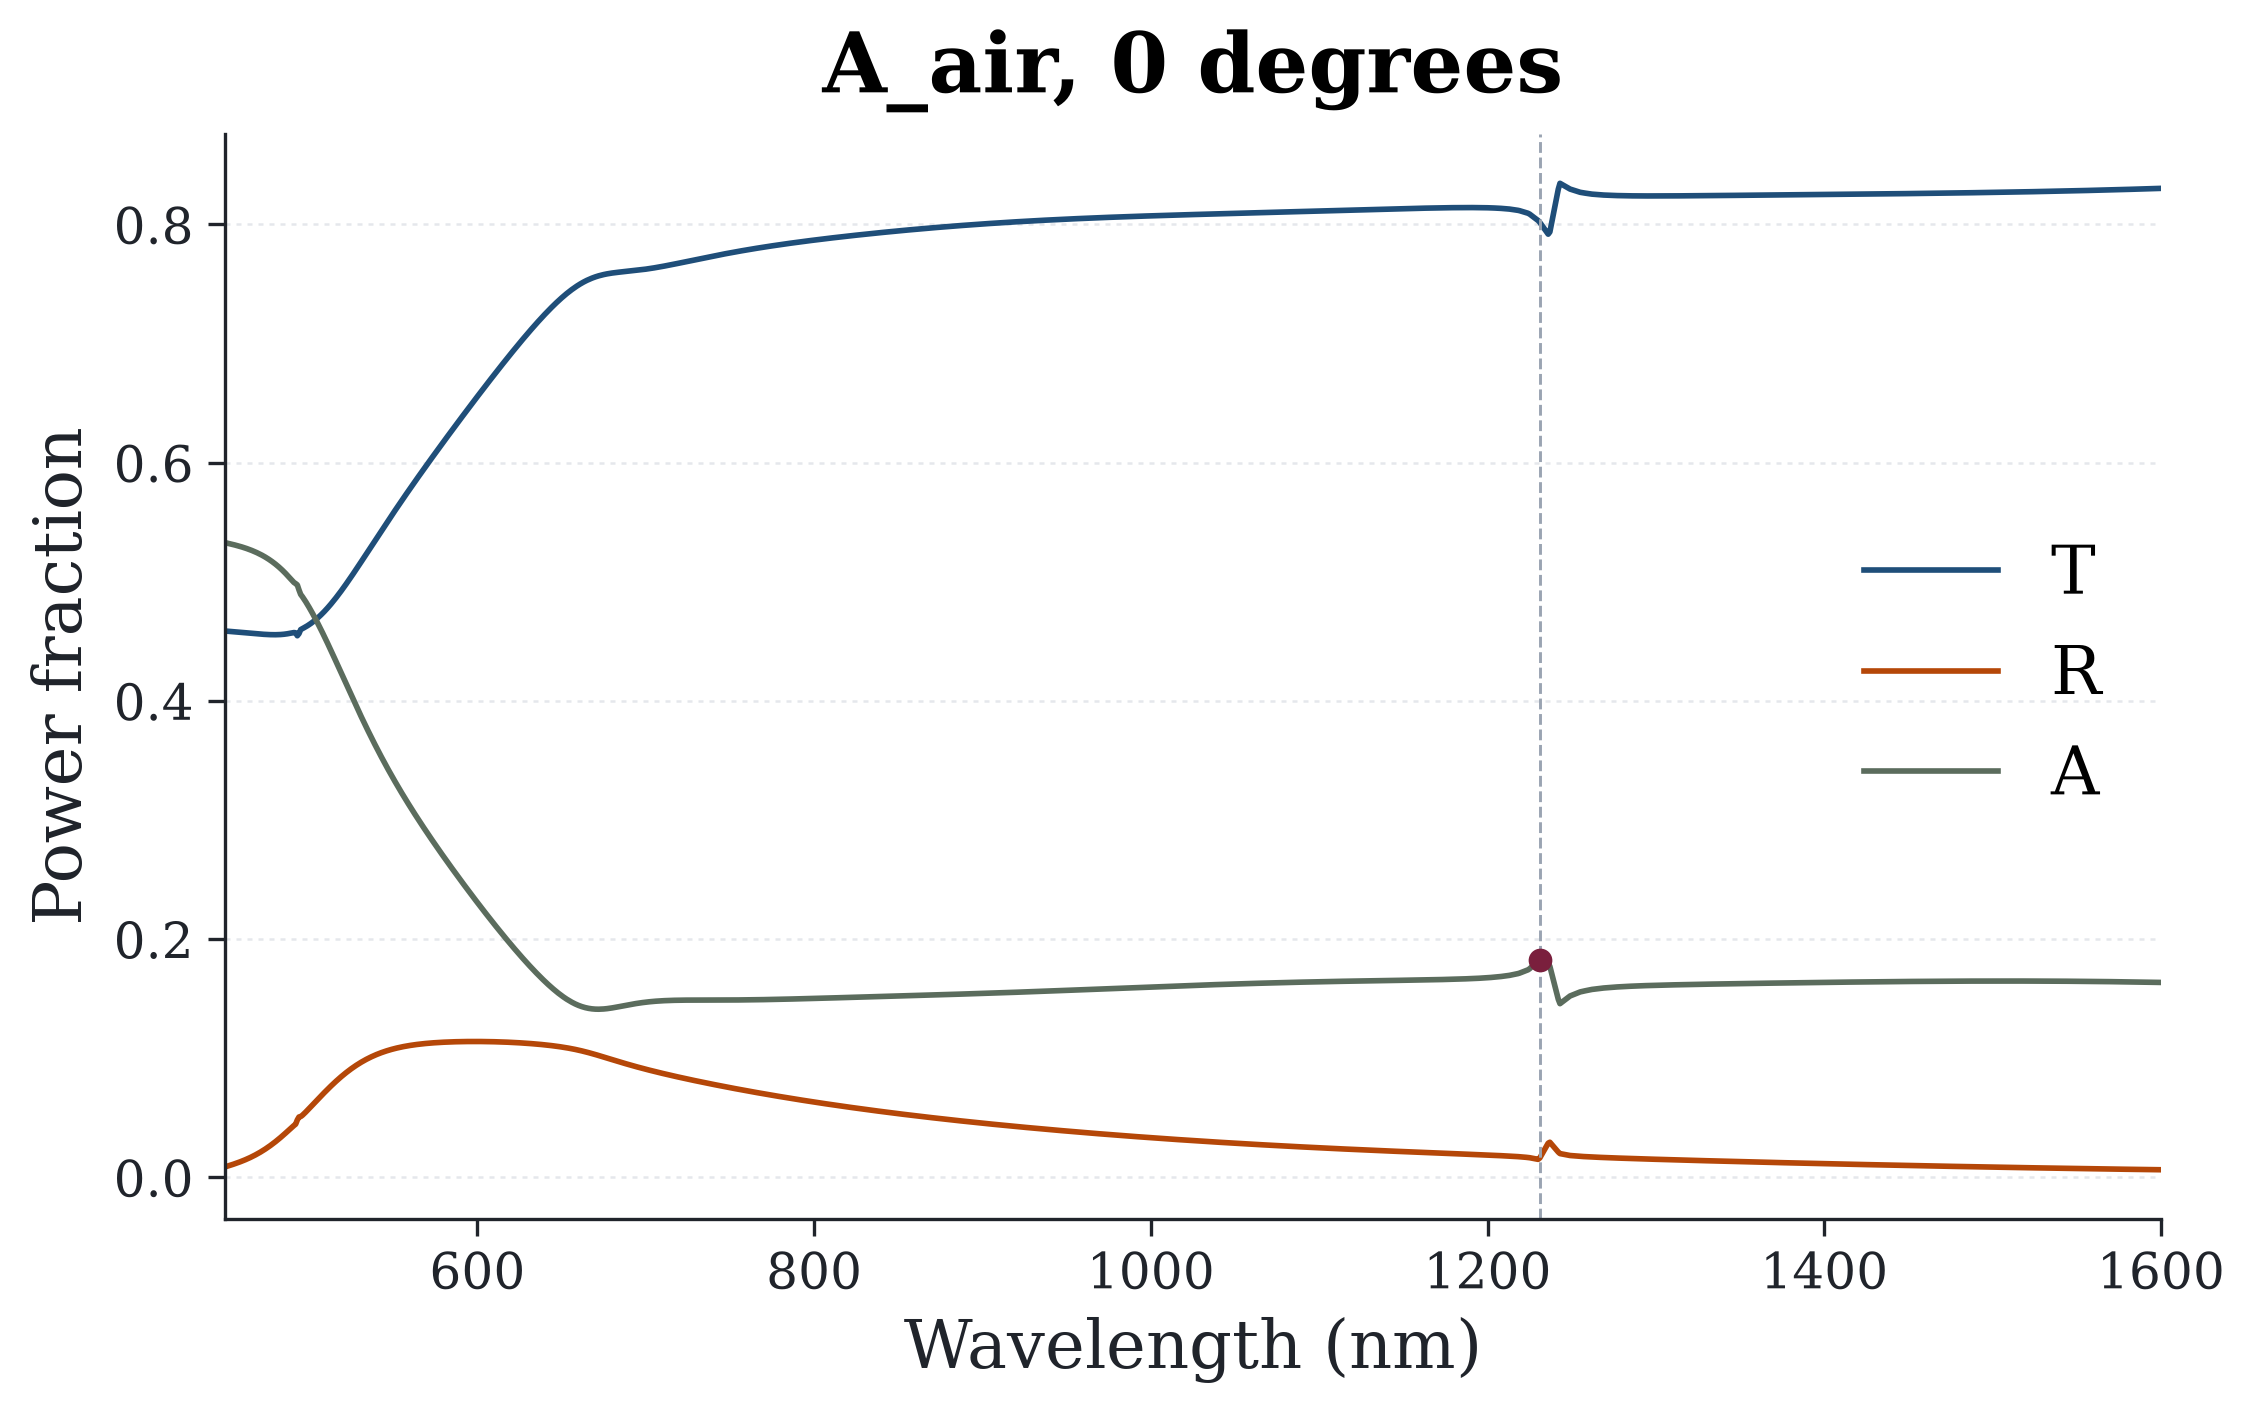
\includegraphics[width=\linewidth,height=0.50\textheight,keepaspectratio]{results/hfss_deliverables/resonances/A_air_0deg_TRA.png}
    \small HFSS: ar, $0^\circ$
  \end{column}
\end{columns}
\vspace{0.12cm}
\small FDTD marca M1 em 772 nm pelo vale de $T$/pico de $R$; HFSS apresenta um pico de $A$ em 1231 nm.
\end{frame}

\begin{frame}{Comparação: estabilidade e próximos passos}
\begin{columns}[T,onlytextwidth]
  \begin{column}{0.49\textwidth}
    \begin{block}{Lumerical FDTD}\small
      Os 12 casos atingiram 10 ps sem o auto-shutoff desejado. Em ângulos oblíquos aparecem valores não físicos de $T$, $R$ ou $A$.
    \end{block}
    \begin{block}{Resultados}\small
      Em $0^\circ$, M1 foi marcada em 772 nm no ar e 905 nm no SiO$_2$. Nos ângulos maiores, os marcadores são exploratórios.
    \end{block}
  \end{column}
  \begin{column}{0.49\textwidth}
    \begin{block}{HFSS}\small
      Os espectros não mostram as grandes divergências observadas no FDTD. Há feições estreitas, especialmente em incidência oblíqua.
    \end{block}
    \begin{block}{Comparação}\small
      Comparar os mesmos extremos e mapas e avaliar a sensibilidade à malha, às portas e à amostragem.
    \end{block}
  \end{column}
\end{columns}
\end{frame}

\end{document}
